% -*- coding: GBK2312 -*-

\chapter{绪论} \label{chpt:A}

\section{人工神经网络技术概述}

%来自wikipedia
按照机器学习以及认知科学领域普遍认同的定义,人工神经网络是一种可以根据外部信息进行自适应的仿生数学模型.如今在计算机相关技术中,人工神经网络是如今在计算机识别和控制、统计规划、医学以及生物研究领域,乃至社会经济等领域都具有广泛应用价值的研究方向.

\subsection{人工神经网络技术的技术渊源}

%以下内容来自
%https://blog.csdn.net/jinking01/article/details/103344186?spm=1001.2101.3001.6650.5&utm_medium=distribute.pc_relevant.none-task-blog-2%7Edefault%7EBlogCommendFromBaidu%7ERate-5.pc_relevant_paycolumn_v3&depth_1-utm_source=distribute.pc_relevant.none-task-blog-2%7Edefault%7EBlogCommendFromBaidu%7ERate-5.pc_relevant_paycolumn_v3&utm_relevant_index=8

人工神经网络技术领域具有很深刻的多学科领域交叉的历史背景,这可以追溯到医学和生物研究领域对人类神经活动的研究模拟. 根据奥地利医生 Franz Joseph Gall 对人类神经活动依赖于人体脑部的功能的论断, 人类对神经活动的研究进入正轨. 而意大利细胞学家 Camillo Golgi 发明的 Golgi染色法 通过对脑组织切片进行染色并观测其微观结构, 确立了对人体神经网络的微观研究方式.西班牙神经组织学家 Santiago Ramón y Cajal 在此基础上进一步改进染色技术,并通过大量实验确认了神经细胞中神经元功能和结构的独立性.

1943年,基于 Golgi 和 Cajal 对生物神经系统运行原理的一系列深入研究, Warren McCulloch 和 Walter Pitts 首次提出借鉴已知神经细胞运行机制的数学模型 M-P 模型.

\begin{figure}
	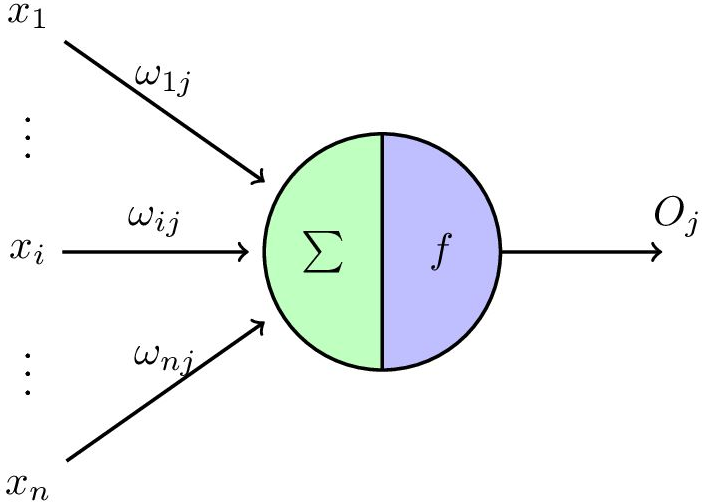
\includegraphics[scale=0.7]{Figures/mpmodel.png}
	\caption{M-P 模型}
\end{figure}
\begin{figure}
	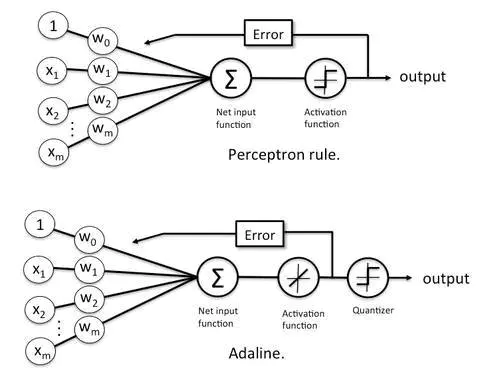
\includegraphics[scale=0.7]{Figures/perceptron.png}
	\caption{Perceptron 模型}
\end{figure}


M-P模型的提出证明仿神经网络的数学模型在一定程度上可以实现逻辑和算术函数的功能.而20世纪40年代末的 Donald Olding Hebb 通过在数学模型中引入对神经元的激活机制的抽象, 提出了调整其数学模型参数的 Hebb 学习规则, 以模拟神经元的选择性和差异性的激发来模拟生物神经元对外界刺激的学习机制. 与1986年提出的基于神经网络已知输入输出 Delta 学习规则相比, Hebb规则被称为无监督学习的重要机制, 而后者则是有监督学习的重要规则.

1958年,Cornell 航空实验室的 Frank Rosenblatt 发明的简单二分类器神经网络,即"感知器"人工神经网络 Perceptron 引发了学界对神经网络结构和相关学习算法的广泛深入研究.

